% Los listados y las referencias contienen operadores y guiones propios de
% SystemVerilog; las declaraciones de alineación pertenecen a los flotantes.
% chktex-file 1
% chktex-file 8

\section{Criterio de validación}

La verificación se organiza con la misma separación que el diseño.
Primero se comprueba el cálculo combinacional; luego, el ingreso de
una señal asíncrona al dominio del reloj; y finalmente, el recorrido
completo desde los controles hasta los LEDs. De esta
manera, una falla
puede asociarse con una responsabilidad concreta antes de analizar el conjunto.

El análisis estático complementó esas pruebas. En la ejecución
documentada, el panel \textit{Linter} de \tech{Vivado} no informó
violaciones ni reglas exceptuadas. Este resultado respalda la calidad
de la descripción, aunque no demuestra por sí mismo que las
operaciones sean correctas. La figura~\ref{fig:linter} documenta esta
ejecución.

\begin{figure}[H]
	\centering
	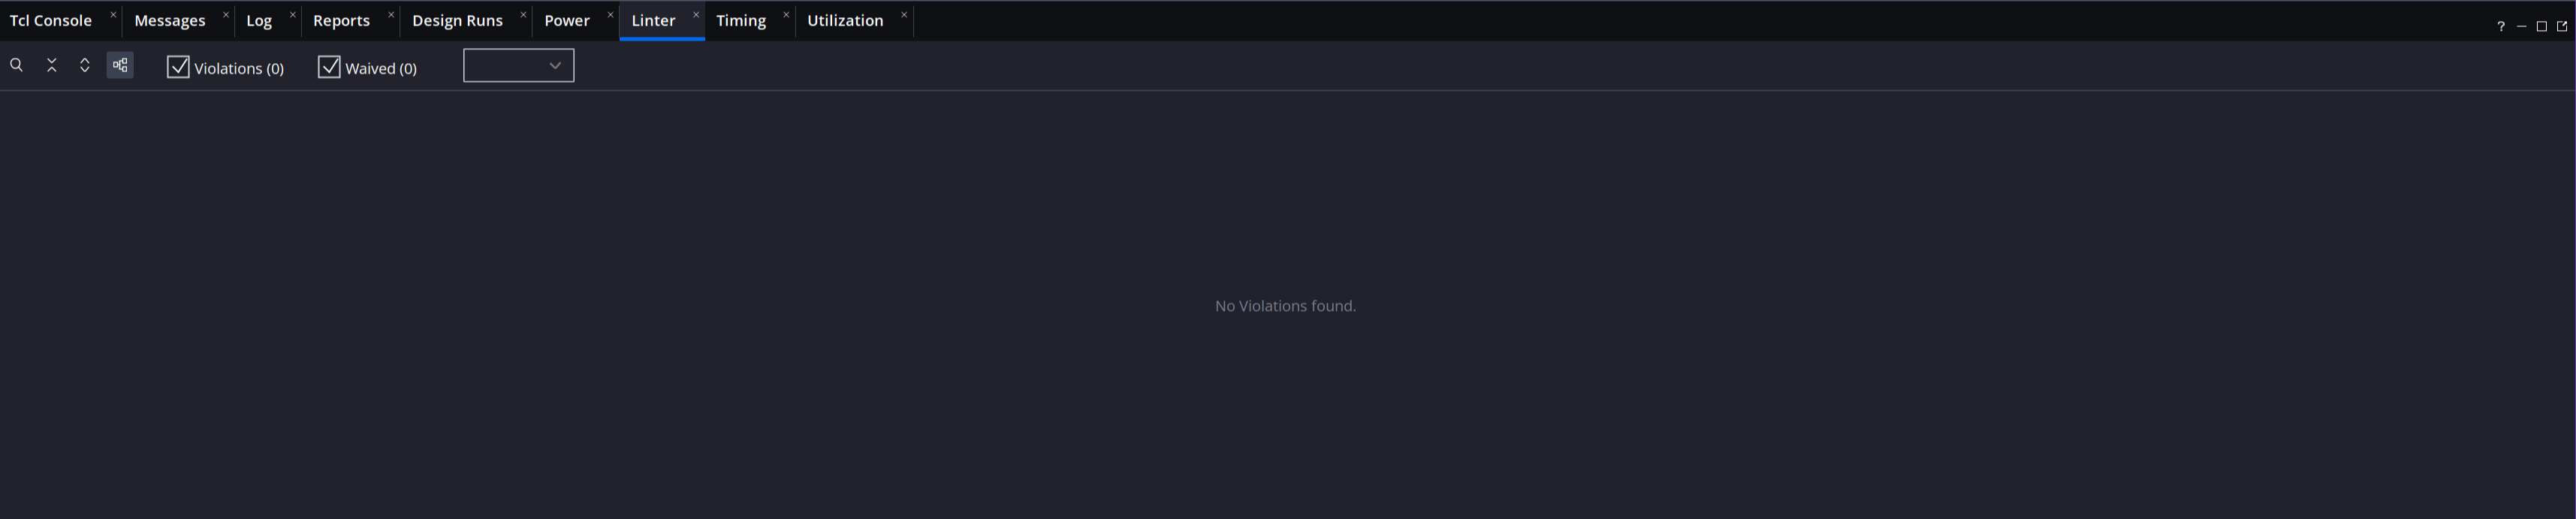
\includegraphics[width=\textwidth]{img/linter_successful.png}
	\caption{Análisis estático de Vivado sin violaciones reportadas.}%
	\label{fig:linter}
\end{figure}

La tabla~\ref{tab:trazabilidad} relaciona los requisitos principales
con el módulo que los implementa y la evidencia utilizada.

\begin{table}[H]
	\centering
	\small
	\begin{tabularx}{\textwidth}{L{3.5cm}L{2.8cm}L{3.5cm}Y}
		\toprule
		\textbf{Requisito} & \textbf{Módulo} & \textbf{Verificación} &
		\textbf{Evidencia} \\
		\midrule
		Ejecutar ocho operaciones & \texttt{alu} & \texttt{alu\_tb} & Casos
		dirigidos y 100 pares pseudoaleatorios por operación. \\
		Generar Z, C y V & \texttt{alu} & \texttt{alu\_tb} & Fronteras con
		y sin signo y comparación con un modelo ampliado. \\
		Sincronizar pulsadores & \texttt{button\_input} &
		\texttt{button\_input\_tb} & Activación y liberación observadas
		después de dos flancos. \\
		Cargar y conservar entradas & \texttt{alu\_top} &
		\texttt{alu\_top\_tb} & Cargas individuales, simultáneas y botón sostenido. \\
		Priorizar el reset & \texttt{alu\_top} & \texttt{alu\_top\_tb} &
		Reset aplicado junto con las tres cargas. \\
		Depender del reloj & \texttt{alu\_top} & \texttt{alu\_top\_tb} &
		Registros conservados con el reloj detenido. \\
		Cumplir \SI{100}{\mega\hertz} & Diseño implementado & Timing
		post-route & WNS, WHS y WPWS positivos en las rutas restringidas. \\
		\bottomrule
	\end{tabularx}
	\caption{Trazabilidad entre requisitos y evidencia de verificación.}%
	\label{tab:trazabilidad}
\end{table}

\section{Verificación de la ALU}

\subsection{Criterio y estímulos}

Verificar la ALU exige algo más que comprobar que aparezca un valor en
la salida. Es necesario confirmar, por un lado, que cada opcode
seleccione la operación prevista y, por otro, que los indicadores Z, C
y V conserven su significado en los casos límite.

El banco \texttt{alu\_tb.sv} organiza cada ensayo mediante la tarea
\texttt{check\_result}. La tarea presenta A, B y el opcode, deja
transcurrir \SI{10}{\nano\second} para que se estabilice la lógica
combinacional y recién entonces contrasta la respuesta completa con un
modelo de referencia. La comparación utiliza \texttt{!==}; por eso un
bit desconocido no puede pasar inadvertido como si fuera un resultado
válido.

El modelo de referencia está planteado, además, para no repetir
literalmente las expresiones utilizadas por el circuito. Si ambos
lados resolvieran cada condición de
la misma manera, un error podría quedar reproducido tanto en el diseño
como en la prueba. Para calcular el overflow, por ejemplo, los operandos
se extienden con signo a nueve bits. La suma ampliada puede compararse
entonces con los límites \num{-128} y \num{127} sin perder el desbordamiento que se
quiere detectar. El circuito obtiene el mismo indicador mediante los
bits de signo, de modo que ambas implementaciones llegan al resultado
por caminos diferentes.

Con el carry se aplica el mismo criterio de independencia. El modelo
determina que existe acarreo cuando A supera el valor que resulta de
restar B al máximo sin signo. Por su parte, la ALU conserva el noveno
bit de la suma. Así, el testbench no solo compara resultados, sino también dos
formas equivalentes de interpretar sus condiciones de borde.

\begin{codebox}[language=SystemVerilog]
	signed_a = {test_a[NB_DATA-1], test_a};
	signed_b = {test_b[NB_DATA-1], test_b};

	expected = test_a + test_b;
	expected_carry = test_a > (ALL_ONES - test_b);
	signed_result = signed_a + signed_b;
	expected_overflow =
	(signed_result < SIGNED_MIN) ||
	(signed_result > SIGNED_MAX);
\end{codebox}

La secuencia incluye 14 casos dirigidos: resultado cero, carry,
fronteras positivas y negativas, desplazamientos, NOR y opcode
inválido. A continuación se generan cien pares de operandos para cada
una de las ocho operaciones. La semilla fija \texttt{32'h1a2b3c4d}
permite repetir exactamente los 800 estímulos pseudoaleatorios.

\subsection{Resultado observado}

La figura~\ref{fig:wave-alu} muestra el comienzo de la ejecución.
\texttt{FF + 01} entrega \texttt{00}, con Z y C activos; luego, el
mismo patrón \texttt{80} desplazado una posición produce \texttt{C0}
con SRA, mientras que con SRL da \texttt{40}. La diferencia entre
ambas salidas hace visibles tres
propiedades diferentes sin depender todavía de los estímulos aleatorios.

\begin{figure}[H]
	\centering
	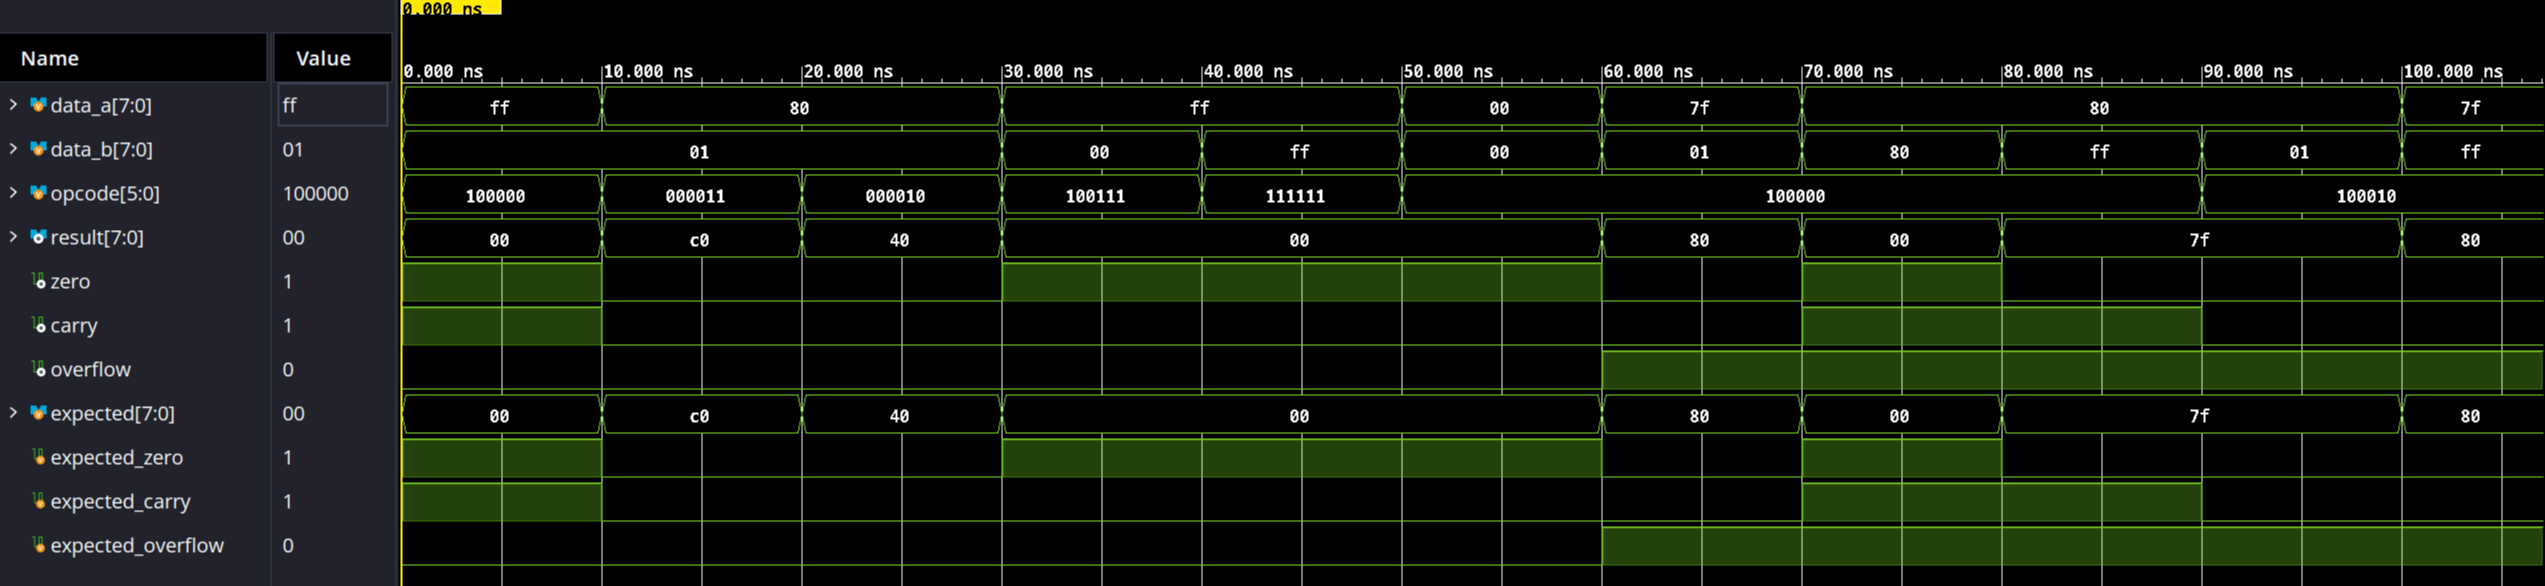
\includegraphics[width=\textwidth]{img/waveforms_alu.png}
	\caption{Primeros casos dirigidos de la ALU y sus indicadores.}%
	\label{fig:wave-alu}
\end{figure}

La comparación automática continuó durante toda la simulación. La
consola confirmó que las 814 comprobaciones terminaron sin errores a
los \SI{8140}{\nano\second}. El cierre de la ejecución puede verse en
la figura~\ref{fig:test-alu}.

\begin{figure}[H]
	\centering
	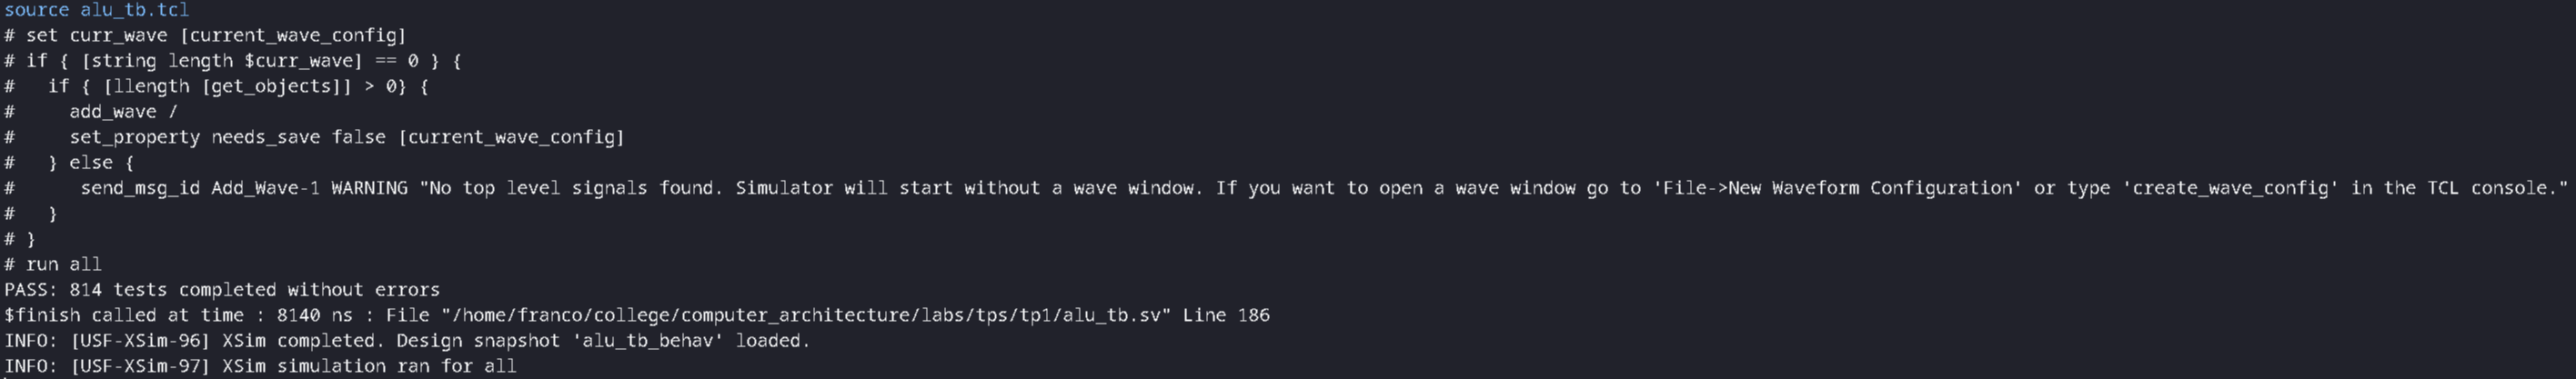
\includegraphics[width=\textwidth]{img/testbench_alu.png}
	\caption{Finalización de las 814 comprobaciones de la ALU.}%
	\label{fig:test-alu}
\end{figure}

\subsection{Interpretación}

El resultado confirma que las ocho ramas, el caso inválido y las
combinaciones dirigidas de Z, C y V coinciden con el modelo
utilizado. Las pruebas pseudoaleatorias amplían la variedad de
operandos, mientras que los casos de frontera aseguran que no se
dependa del azar para alcanzar los escenarios más importantes. No se
trata de una enumeración exhaustiva de las $2^{22}$ combinaciones
posibles de A, B y opcode, pero sí de una cobertura dirigida y
reproducible de las propiedades definidas.

\section{Verificación del sincronizador}

\subsection{Criterio y estímulos}

La prueba de \texttt{button\_input} busca demostrar que la salida no
sigue al pin de manera inmediata, sino después de atravesar las
dos etapas. El testbench genera un reloj de \SI{10}{\nano\second},
modifica el botón en flancos descendentes y observa la salida después
de cada flanco ascendente. También aplica un nivel sostenido, la
liberación y una pulsación de un solo ciclo.

\subsection{Resultado observado}

En la figura~\ref{fig:wave-button}, la entrada se activa a los
\SI{10}{\nano\second}. La primera etapa la captura a los
\SI{15}{\nano\second} y la salida cambia a los \SI{25}{\nano\second}.
Al liberar el botón a los \SI{80}{\nano\second}, la salida vuelve a
cero a los \SI{95}{\nano\second}. Las 14 comprobaciones finalizaron
sin errores a los \SI{126}{\nano\second}.

\begin{figure}[H]
	\centering
	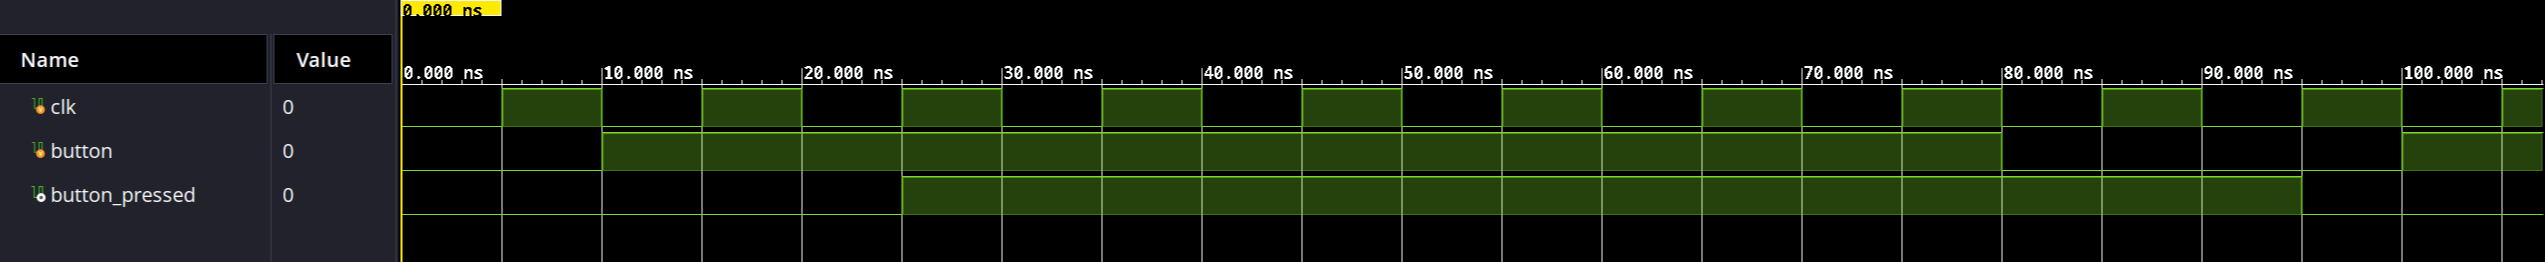
\includegraphics[width=\textwidth]{img/waveforms_button.png}
	\caption{Propagación del nivel por las dos etapas del sincronizador.}%
	\label{fig:wave-button}
\end{figure}

\begin{figure}[H]
	\centering
	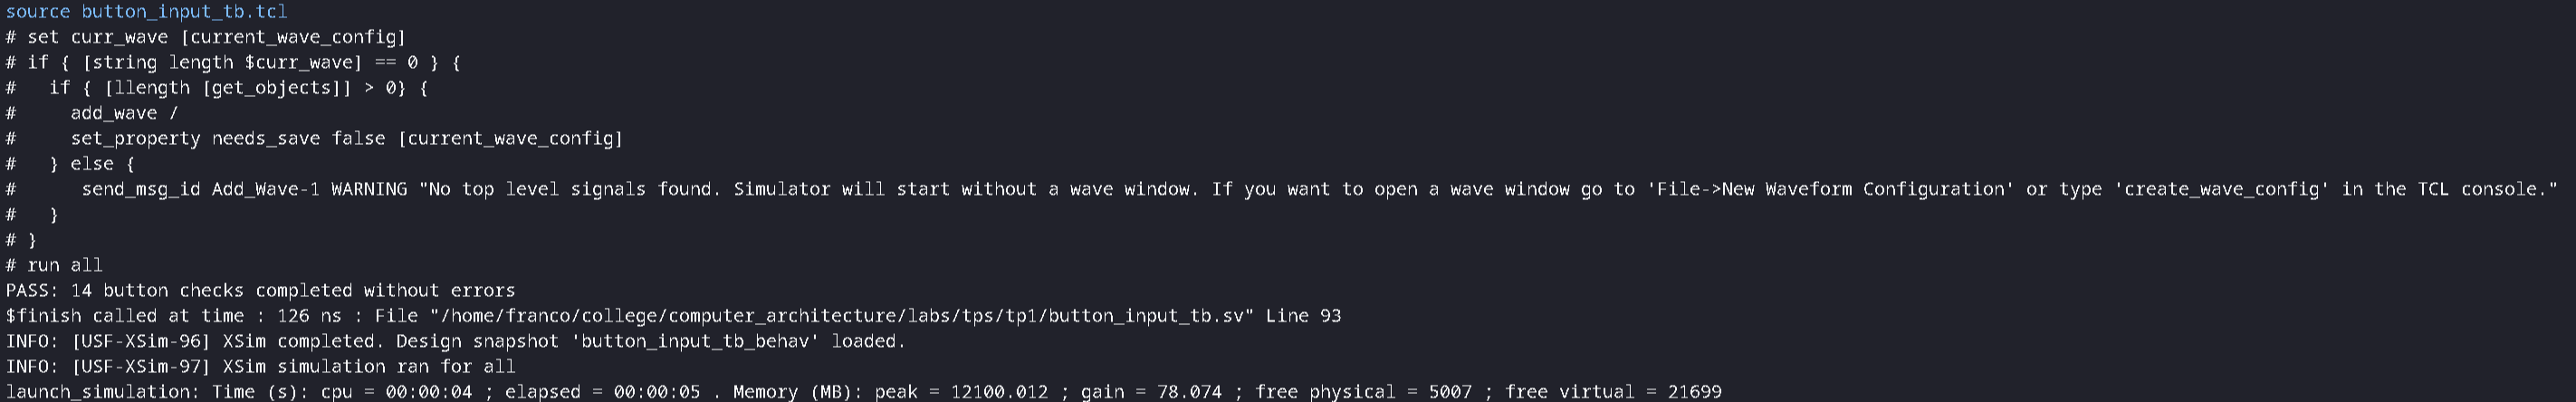
\includegraphics[width=\textwidth]{img/testbench_button.png}
	\caption{Finalización de las 14 comprobaciones del sincronizador.}
\end{figure}

\subsection{Interpretación}

La secuencia observada coincide con dos registros conectados en serie
y con las asignaciones no bloqueantes utilizadas. La simulación
comprueba el retardo lógico y la conservación de niveles; no
reproduce la metastabilidad eléctrica que motiva la estructura ni
permite medir su probabilidad. Tampoco demuestra un filtrado de
rebotes, porque el módulo no cumple esa función.

\section{Verificación de la integración}

\subsection{Criterio y estímulos}

El último banco de pruebas se ocupa de la integración. Comprueba que
cada valor presentado en los switches llegue al registro correcto y
que el resultado aparezca en los LEDs. En cada paso
compara simultáneamente A, B, opcode y los once bits de salida. Así
puede distinguir un error de cálculo de una carga equivocada.

La secuencia ensaya el estado inicial, cambios de switches sin
pulsación, cargas individuales, botones sostenidos, rebotes
simulados, carga simultánea de A y B, prioridad del reset y
recuperación posterior. También detiene el reloj durante una
solicitud de carga para comprobar que los registros conserven su
estado hasta que vuelvan los flancos.

El testbench reserva tres ciclos para cada carga: dos para que el
nivel atraviese el sincronizador y uno adicional para que el registro
observe la habilitación ya actualizada. Esta espera reproduce el
comportamiento de los bloques secuenciales y no es un retardo
arbitrario agregado a la prueba.

\subsection{Resultado observado}

La figura~\ref{fig:wave-top} presenta la inicialización y el comienzo
de la carga de A. Mientras el opcode permanece en cero, los ocho bits
de resultado son nulos y \texttt{leds} muestra \texttt{100}
hexadecimal, correspondiente a Z activo. El contador de errores
permanece en cero.

\begin{figure}[H]
	\centering
	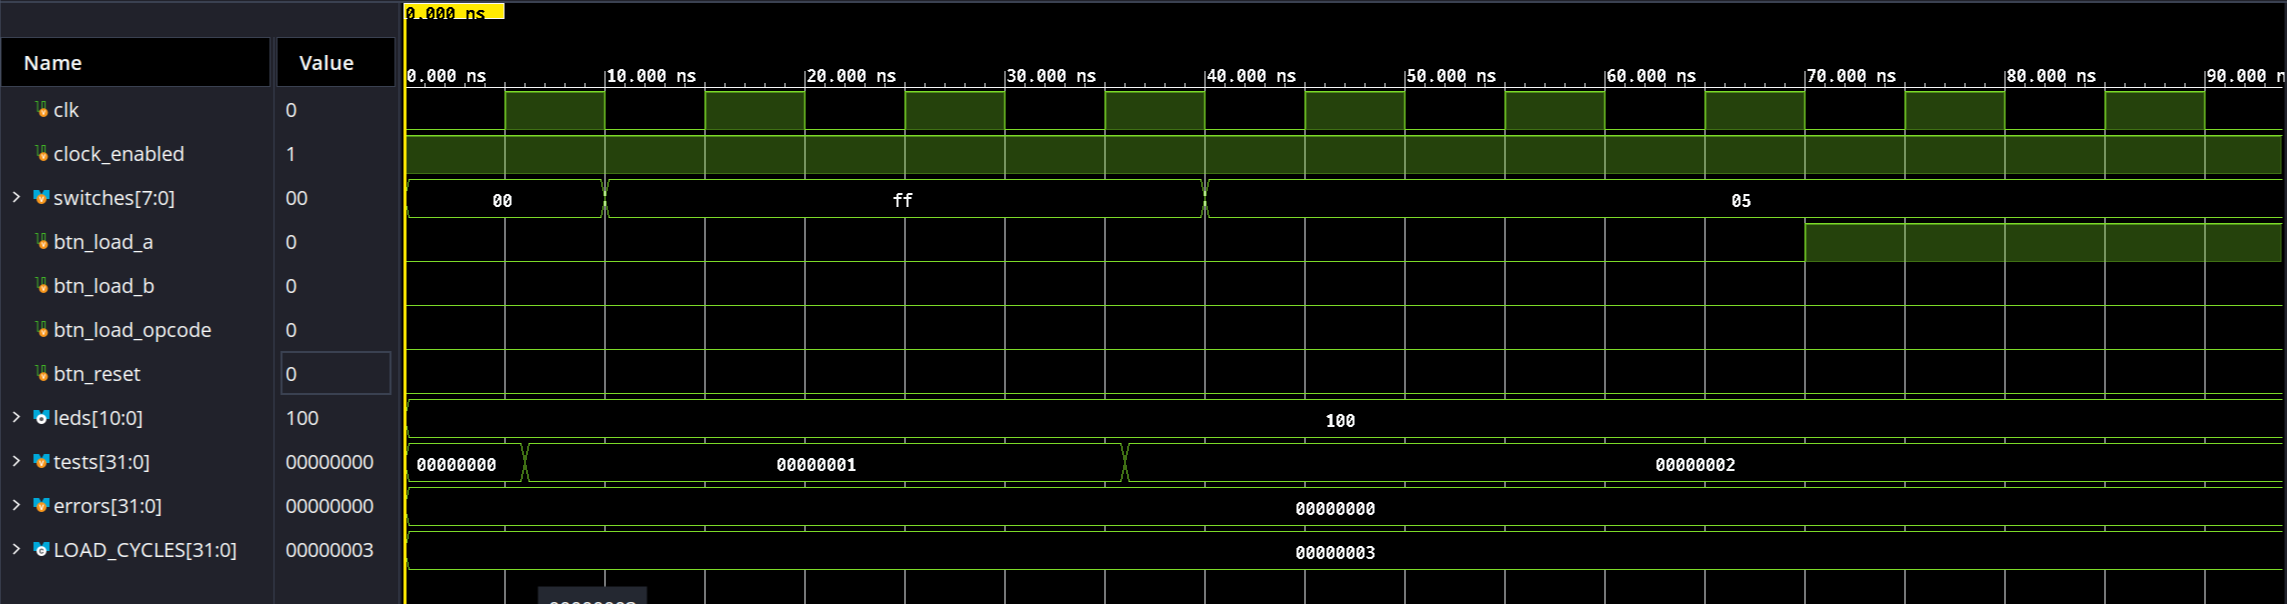
\includegraphics[width=\textwidth]{img/waveforms_top.png}
	\caption{Inicialización y comienzo de una carga en el módulo superior.}%
	\label{fig:wave-top}
\end{figure}

Fuera de la ventana visible se aplicaron operaciones conocidas para
encender y apagar cada indicador, se verificó el reset desde
registros no nulos y se comprobó que el sistema pudiera volver a
operar después del borrado. La ejecución concluyó sin errores después
de 38 comprobaciones, a los \SI{7051}{\nano\second}.

\begin{figure}[H]
	\centering
	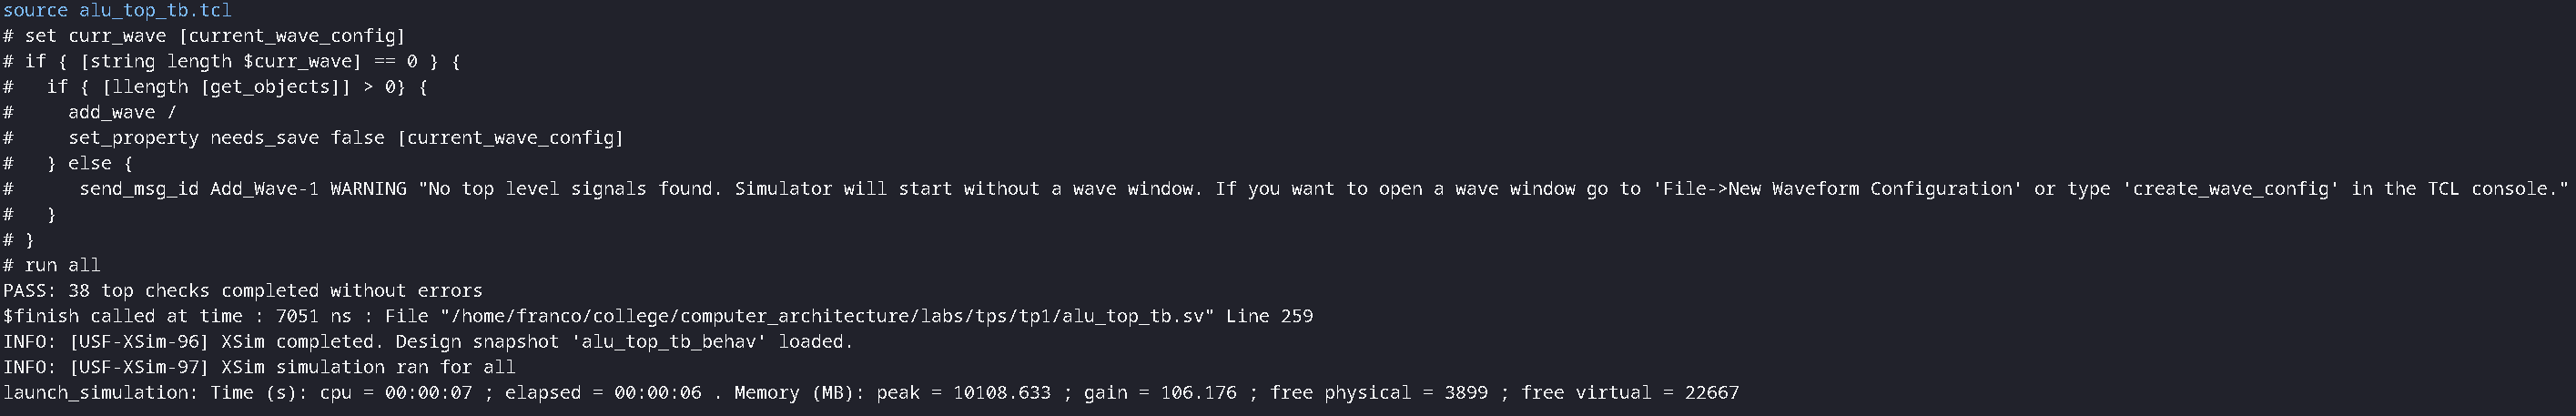
\includegraphics[width=\textwidth]{img/testbench_top.png}
	\caption{Finalización de las 38 comprobaciones de integración.}
\end{figure}

\subsection{Interpretación}

Estas pruebas enlazan las responsabilidades verificadas previamente:
los pulsadores se propagan con el retardo previsto, los registros
capturan y conservan los datos, el reset prevalece sobre las cargas y
la ALU actualiza los LEDs. En conjunto, los tres bancos
completaron 866 comprobaciones sin errores.
